 \documentclass[xcolor=dvipsnames,table]{beamer}

\usepackage{latexsym}
\usepackage[utf8]{inputenc}
\usepackage[brazil]{babel}
\usepackage{amssymb}
\usepackage{amsmath}
\usepackage{stmaryrd}
\usepackage{fancybox}
\usepackage{datetime}
\usepackage[T1]{fontenc}
\usepackage{graphicx}
\usepackage{graphics}
\usepackage{url}
\usepackage{algorithmic}
\usepackage{algorithm}
\usepackage{acronym}
\usepackage{array}

\usepackage{enumitem}

\newtheorem{definicao}{Definio}
\newcommand{\tab}{\hspace*{2em}}

\mode<presentation>
{
  \definecolor{colortexto}{RGB}{0,0,0}
 
  \setbeamertemplate{background canvas}[vertical shading][ bottom=white!10,top=white!10]
  \setbeamercolor{normal text}{fg=colortexto} 

  \usetheme{Warsaw}
}

\title{Informática na Educação}  

\author{
  Esdras Lins Bispo Jr. \\ \url{bispojr@ufj.edu.br}
  } 
 \institute{
  Tópicos em Informática e Educação \\Bacharelado em Ciência da Computação}
\date{\textbf{27 de agosto de 2026} }

\logo{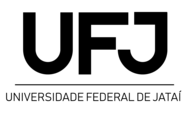
\includegraphics[width=1.5cm]{images/ufjJataiLogo.png}}

\begin{document}

	\begin{frame}
		\titlepage
	\end{frame}

	\AtBeginSection{
		\begin{frame}{Sumário}%[allowframebreaks]{Sumário}
    		\tableofcontents[currentsection]
    		%\tableofcontents[currentsection, hideothersubsections]
		\end{frame}
	}

	\begin{frame}{Plano de Aula}
		\tableofcontents
		%\tableofcontents[hideallsubsections]
	\end{frame}
	
	\section{Instrução pelos Colegas}

        \begin{frame}{Pesquisa 002}
		\begin{block}{[P002]}
			Como foi a leitura do estudo prévio?
		\end{block}
		\begin{enumerate}[label=(\Alph*)]
			\item Boa leitura
			\item Leitura razoável
			\item Difícil de ler
			\item Não consegui ler
		\end{enumerate}
	\end{frame}

    \begin{frame}{Questão 007}

		\small

    \begin{block}{[Q007]}
    
    Um professor disponibiliza um vídeo sobre determinado conteúdo. Em seguida, faz uma aula em que os estudantes podem fazer perguntas, mas todas as perguntas são respondidas pelo professor e, ao final, os estudantes precisam reproduzir as definições apresentadas no vídeo.

    Considerando a discussão de Valente, qual interpretação é \textbf{mais adequada}?

    \end{block}

    \begin{enumerate}[label=(\Alph*)]

        \item A aula deixou de ser bancária porque houve interação entre professor e estudantes.
        
		\item A aula é necessariamente construcionista porque utiliza uma tecnologia digital.

        \item A aula ainda pode manter uma lógica de transmissão, pois interação, por si só, não garante construção de conhecimento.

        \item A aula deixou de ser bancária porque os estudantes receberam mais informação do que receberiam em uma aula tradicional.

    \end{enumerate}

\end{frame}

 \begin{frame}{Questão 008}

	\footnotesize

    \begin{block}{[Q008]}
    
    Uma universidade decide ensinar um conceito científico já consolidado. Um professor argumenta:

    \begin{quote}
    ``Esse conhecimento já foi produzido pelos cientistas. Portanto, não faz sentido pedir aos estudantes que o reconstruam; basta apresentá-lo corretamente para que eles o aprendam.''
    \end{quote}

    Qual resposta melhor representa a posição discutida por Valente?

    \end{block}

    \begin{enumerate}[label=(\Alph*)]

        \item O professor está correto: todo conhecimento científico deve ser transmitido, pois reconstruí-lo seria repetir desnecessariamente o trabalho dos cientistas.

        \item O professor está parcialmente correto: o conhecimento já produzido pode ser apresentado ao estudante, mas sua apropriação não ocorre necessariamente por transmissão.

        \item O professor está incorreto: para aprender ciência, cada estudante precisa reproduzir exatamente o percurso histórico dos cientistas.

        \item O professor está incorreto: conhecimento científico não deve ser apresentado ao estudante, apenas descoberto por ele.

    \end{enumerate}

\end{frame}

    \begin{frame}{Questão 009}

		\footnotesize

    \begin{block}{[Q009]}
    
    Dois estudantes estão discutindo:

    \begin{quote}
    \textbf{Estudante 1:} ``Se uma pessoa consegue acessar, interpretar e atribuir significado a uma informação sozinha, então comunicação e educação fazem exatamente a mesma coisa.''

    \textbf{Estudante 2:} ``Não necessariamente. A educação tem uma responsabilidade específica relacionada à construção de conhecimento pelo aprendiz.''
    \end{quote}

   Quem está mais próximo da posição de Valente?

    \end{block}

    \begin{enumerate}[label=(\Alph*)]

        \item O estudante 1, porque toda construção de conhecimento é um processo exclusivamente comunicacional.

        \item O estudante 2, porque Valente atribui à educação o papel de auxiliar e mediar a construção de conhecimento do aprendiz.

        \item O estudante 1, porque interpretar uma informação já é suficiente para caracterizar uma ação educacional.

        \item Os dois estão equivocados, porque Valente considera comunicação e educação áreas indistinguíveis.

    \end{enumerate}

\end{frame}

\begin{frame}{Questão 010}

    \begin{block}{[Q010]}

    Uma professora quer utilizar uma simulação digital para ensinar
    um determinado fenômeno. Ela pode apresentar primeiro a fórmula
    e usar a simulação para confirmar os resultados, ou permitir que
    os estudantes explorem diferentes situações e reflitam sobre
    os resultados observados.

    Qual das propostas é mais consistente com o papel atribuído
    às TDICs por Valente?

    \end{block}

    \begin{enumerate}[label=(\Alph*)]

        \item Apresentar a teoria e usar a simulação para confirmar resultados.       

        \item Usar a simulação para substituir a explicação teórica.
        
		 \item Explorar o fenômeno e usar os resultados para rever explicações.

        \item Usar a simulação para tornar o conteúdo mais atrativo.

    \end{enumerate}

\end{frame}

\begin{frame}{Questão 011}

    \begin{block}{[Q011]}

    Um professor utiliza TDICs de duas maneiras:

    \begin{itemize}

        \item \textbf{Situação I:} disponibiliza uma aula expositiva
        em vídeo para os estudantes assistirem.

        \item \textbf{Situação II:} propõe que os estudantes utilizem
        uma simulação para testar hipóteses, analisar resultados
        e revisar suas explicações.

    \end{itemize}

    Qual situação explora mais claramente as TDICs como ferramentas
    para a construção de conhecimento, segundo Valente?

    \end{block}

    \begin{enumerate}[label=(\Alph*)]

        \item As duas situações, pois ambas utilizam recursos digitais.
		
		\item A situação I, pois facilita o acesso à informação.

        \item A situação II, pois envolve exploração e reflexão.

        \item Nenhuma das duas, pois TDICs não constroem conhecimento.

    \end{enumerate}

\end{frame}

\section{Próxima Aula}
\begin{frame}{Próxima Aula}
    \begin{block}{Leitura Prévia}
        \begin{itemize}
            \item Vicari, et al. (2018). Pensamento Computacional: Revisão Bibliográfica. Relatório Técnico do Projeto de Avaliação de Tecnologias Educacionais. UFRGS/MEC. Disponível em: \url{https://lume.ufrgs.br/bitstream/handle/10183/197566/001097710.pdf}.  
        \end{itemize}
    \end{block}
    \begin{block}{Páginas}
        \begin{itemize}
        \item Seção 3.1: Bases do Pensamento Computacional (pp. 30-37).
        \end{itemize}
    \end{block}
\end{frame}
	
	\begin{frame}
		\titlepage
	\end{frame}
	
\end{document}